\documentclass[a4paper]{article}
\usepackage{graphicx}
\usepackage{array}
\usepackage{wrapfig,lipsum,booktabs}

\topmargin=0.0in
\headheight=0pt

\begin{document}

%name
\center{\textbf {\underline {\huge{KARTIKEYAN V}}}}


%address and contact information
\begin{flushleft}
{J-902, Haware's Splendor,\hfill{Contact : 9819949776} \\sector-20,Plot-52/56,\hfill{Email ID: vkv.5991@gmail.com}\\ Kharghar, \\Navi mumbai.}
\end{flushleft}


%image
\begin{figure}[h]
\begin{flushright}
\graphicspath{ {images/} }
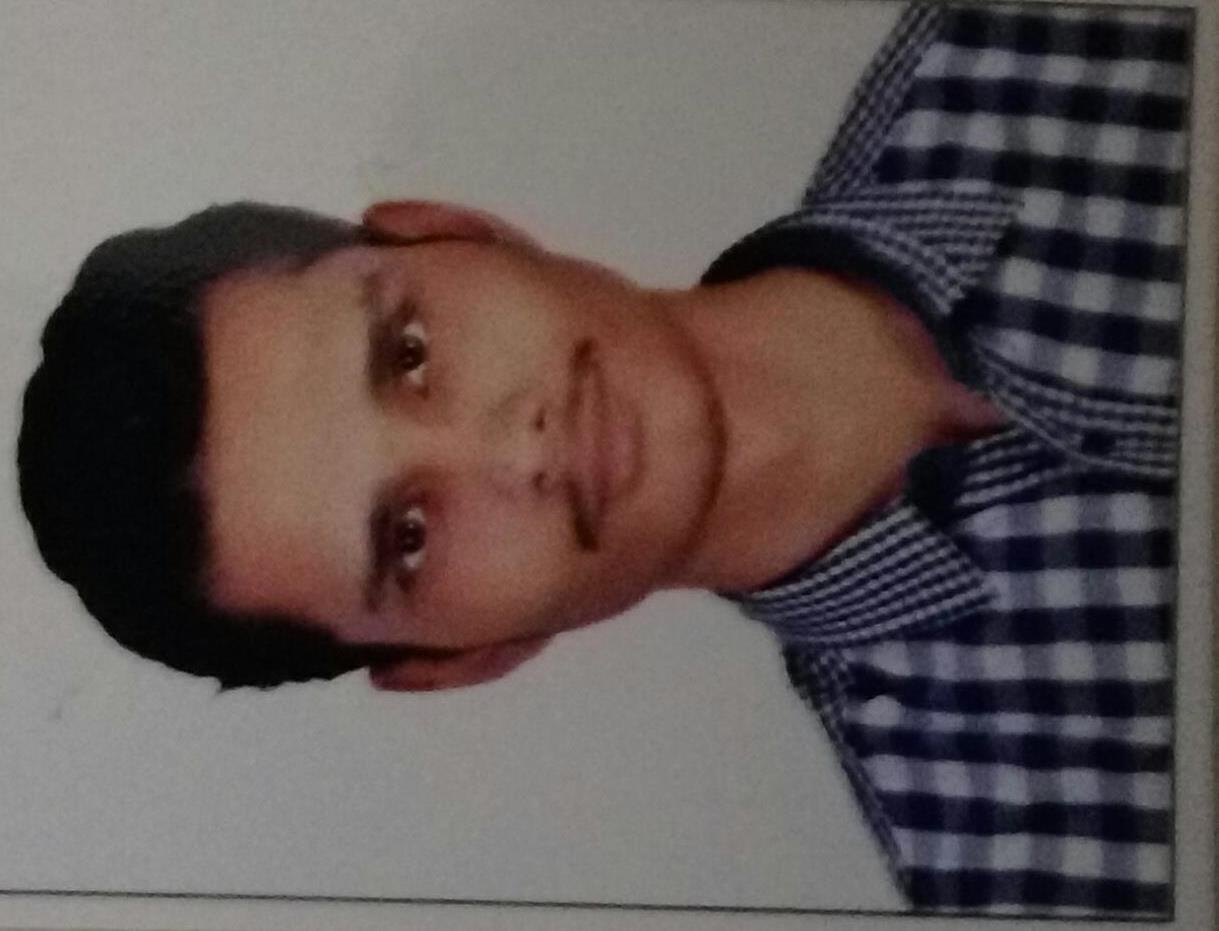
\includegraphics[width=5cm, height=4cm, angle = 270]{cv_pic}
\end{flushright}
\end{figure}


%Carrer objective
\begin{flushleft}
\textbf {CAREER OBJECTIVE}\\
To apply my gained knowledge in the advancement of technology and our society and to have a prosperous future.
\end{flushleft}

%Education
\begin{flushleft}
\textbf { EDUCATION}
\vspace{-5mm}
\begin{center}
\begin{tabular}{ | m{2cm} | m{2.5cm}| m{2cm} | m{2.5cm}| m{3cm} | } 
\hline
Degree& College/School & University & Passing Year & Passing Percentage \\ 
\hline
10th & Abhinav Vidyalay & Mumbai Board & 2011 & 80 \\ 
\hline
12th & Shubham Raje Jr. College & Mumbai Board & 2013 &72.83 \\ 
\hline
B.E & Ramrao Adik Institute of Technology & Mumbai University &2017 & 7.76(till 5th semester) \\
\hline
\end{tabular}
\end{center}
\end{flushleft}

%Projects
\begin{flushleft}
\textbf {PROJECTS}\\
\begin{itemize}
\item	Level 1 wired robotics
\item	Level 2 wireless robotics
\item	Autonomous robotics using Arduino.
\item	Built a  mobile controlled robot which can also work automatically.
\item	Did a project called “Smart Suspensions” for EYIC-2016 Symposium.  
\end{itemize}
\end{flushleft}


%Traning and internships
\begin{flushleft}
\vspace{2in}
\textbf {TRAINING AND INTERNSHIP}\\
\begin{enumerate}
\item  	Attended workshops on:
\begin{itemize}
 \item PCB designing 
\item  Raspberry Pi
\item Advanced Arduino
\end{itemize}
\end{enumerate}
\end{flushleft}

%Research Publications
\begin{flushleft}
\textbf \newline{RESEARCH PUBLICATION}
\end{flushleft}


\begin{flushleft}
\vspace{1in}\textbf {TECHNICAL SKILLS}\\
\begin{enumerate}
\item Programming languages
  \begin{itemize}
      \item C
      \item C++
      \item Assembly language
\end{itemize}
\item Micro controllers
\begin{itemize}
      \item Arduino UNO,Mega,Nano
       \item 8051
\end{itemize}
\end{enumerate}
\end{flushleft}

%Soft Skills
\begin{flushleft}
\textbf {SOFT SKILLS}\\
\begin{itemize}
\item Communication
\item Leadership skills
\item Organizing events
\item Adaptability
\end{itemize}
\end{flushleft}

%Extra Curricular Activities
\begin{flushleft}
\textbf {EXTRA CURRICULAR ACTIVITIES}\\
\begin{enumerate}
\item Sports
\item Making projects related to Electronics
\item Astronomy
\end{enumerate}
\end{flushleft}


%Co-Curricular Activities
\begin{flushleft}
\vspace{2in}
\textbf {CO-CURRICULAR ACTIVITIES}\\
\begin{itemize}
\item Working as a Research team Member with IEEE-RAIT
\item 	Was the Event head for the event of  “Double Dribble”
\item 	Was the lead organiser for the event called “The Ultimate Archer”.
\item 	Was a  faculty assistant for the workshop conducted on Arduino.
\item 	Participated in the 6th National Conference on International Business Management held on 16/09/13 at Dr. D.Y.patil university’s Department of Business management.
\end{itemize}
\end{flushleft}

%Personal Information
\vspace{2mm}
\begin{flushleft}
\begin{tabular}{ cc }
\textbf {Personal Details :  }
 \hfill Fathers Name : & S.Venkatasubramanian  \\ 
 \hfill Mothers Name : & Lakshmi V \\  
 \hfill Sex : & Male   \\ 
 \hfill Date Of Birth : &15/10/1995  \\
 \hfill Nationality : & INDIAN  \\
 \hfill Marital Status : & Single
\end{tabular}
\end{flushleft}








\end{document}